\documentclass[10pt,letterpaper]{article}
\usepackage[utf8]{inputenc}
\usepackage{amsmath}
\usepackage{amsfonts}
\usepackage{amssymb}
\usepackage{graphicx}
\usepackage[left=1cm,right=1cm,top=1cm,bottom=1cm]{geometry}
\author{Derek Steede}
\title{Steady Hands}
\begin{document}
\maketitle

We competed to see who could hold a laser the steadiest on a dot at both a medium and long distance. We used a high speed camera that recorded the area of any pixels of it's images that changed, as well the position of the center of the area. This data was recorded for all five participants in the competition, so we have ten different data sets. 

\vline 

We then found the averages of the x-positions, y-positions, the deviations of these values and the total deviation of the easured values. We then found the distance of each point in the first ten seconds of the competition from the average value and generated histograms of the distances.

\begin{table}
\begin{tabular}{cccccc}
datafile & x-avg & y-avg & x-dev & y-dev & T-dev\\

1 sec & --- & --- & --- & --- & ---\\

201745135431.txt & 497.375 & 577.75 & 3.5229 & 12.9118 & 13.3837\\
20174513521.txt & 495.6667 & 587.3333 & 8.4113 & 11.0708 & 13.9037\\
201745135328.txt & 491.375 & 572.4375 & 4.6961 & 13.2326 & 14.0412\\
201745135944.txt & 506.125 & 574.1875 & 5.534 & 13.6144 & 14.6961\\
201745135111.txt & 498.1875 & 589.8125 & 10.7833 & 13.9334 & 17.6187\\

10 sec & --- & --- & --- & --- & ---\\

20174513577.txt & 472.6667 & 579.5 & 16.2481 & 27.34502 & 31.8080\\
201745135246.txt & 492.25 & 563.0 & 15.0665 & 29.8005 & 33.3927\\
201745135616.txt & 474.8125 & 589.375 & 13.1799 & 30.6416 & 33.356\\
201745135851.txt & 491.625 & 596.9375 & 24.9596 & 32.2462 & 40.7774\\
20174513581.txt & 524.9375 & 598.5625 & 23.0689 & 34.5950 & 41.5811\\

\end{tabular}
\end{table}

\begin{table}
\begin{tabular}{cc}
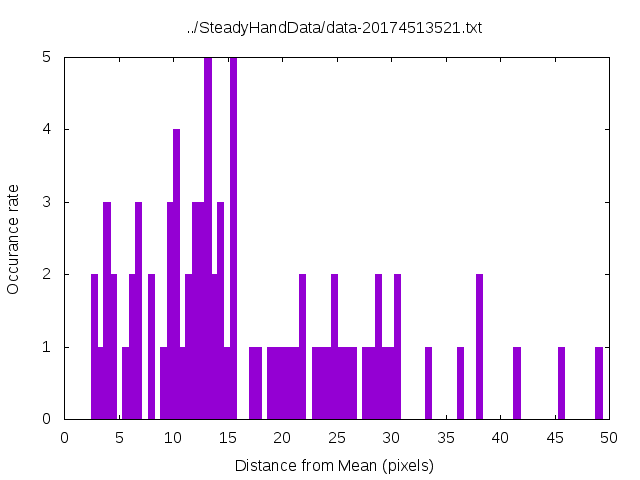
\includegraphics[scale=.5]{graph-data-20174513521.png} & 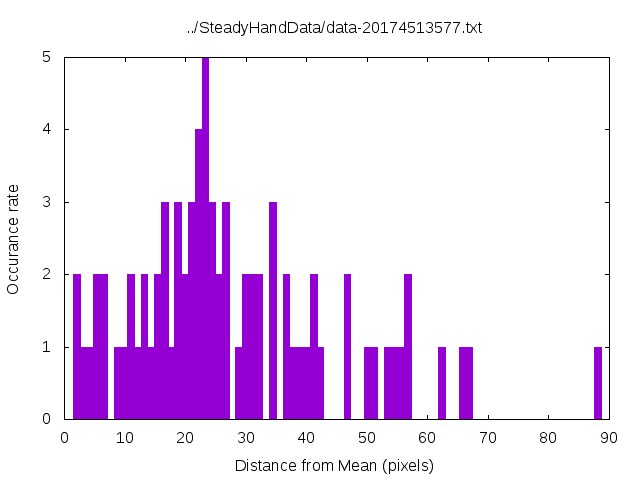
\includegraphics[scale=.5]{graph-data-20174513577.png}\\
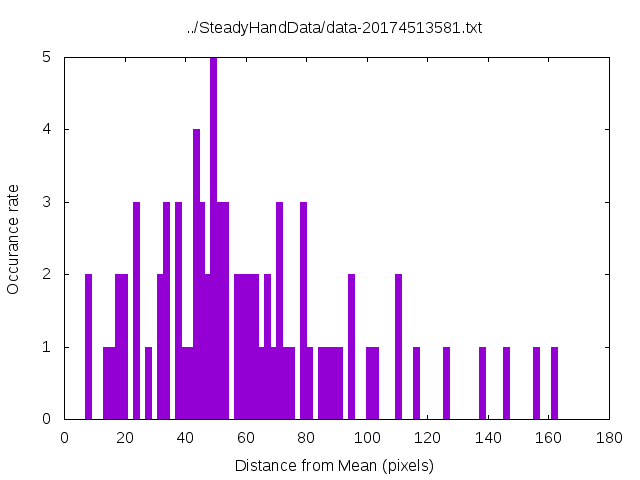
\includegraphics[scale=.5]{graph-data-20174513581.png} & 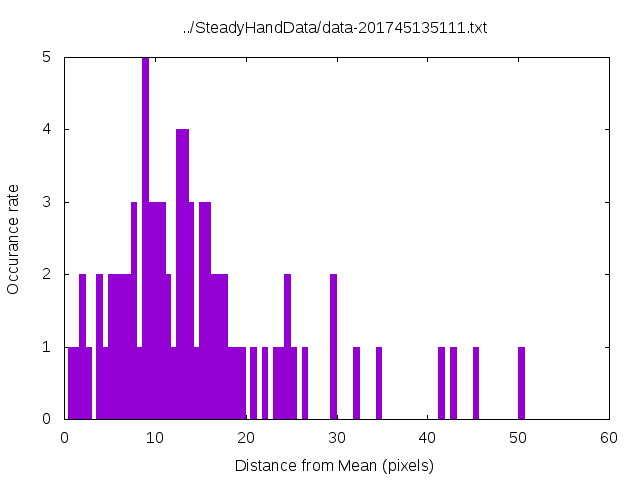
\includegraphics[scale=.5]{graph-data-201745135111.png}\\
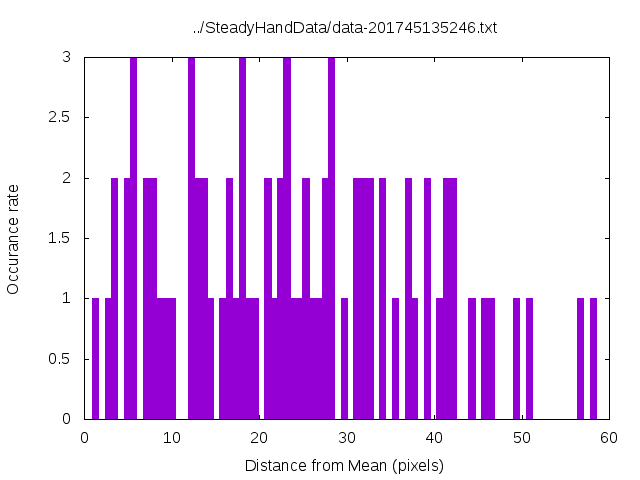
\includegraphics[scale=.5]{graph-data-201745135246.png} & 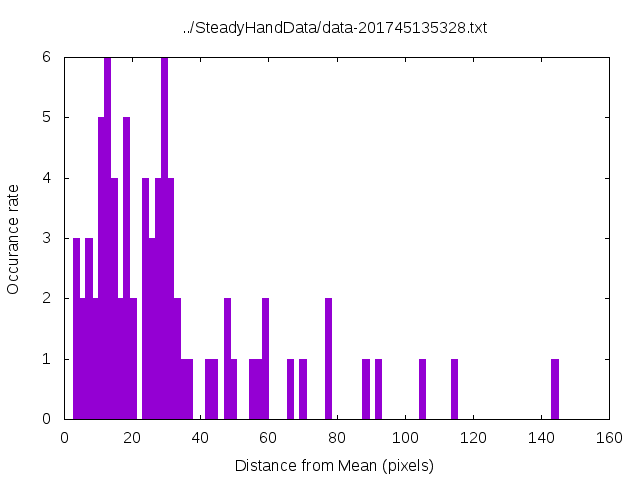
\includegraphics[scale=.5]{graph-data-201745135328.png}\\
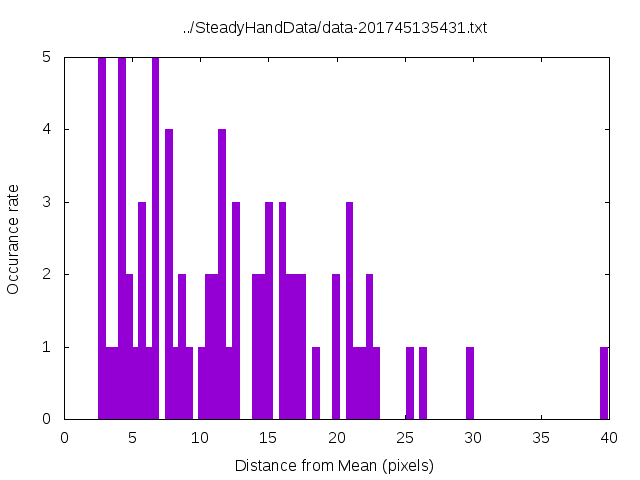
\includegraphics[scale=.5]{graph-data-201745135431.png} & 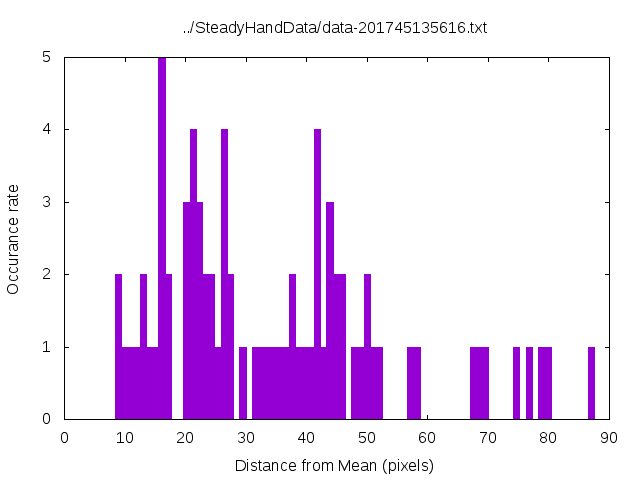
\includegraphics[scale=.5]{graph-data-201745135616.png}\\
\end{tabular}
\end{table}

\begin{table}
\begin{tabular}{cc}
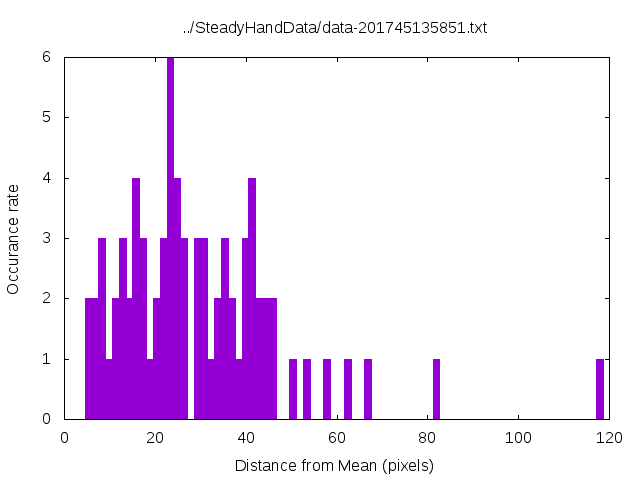
\includegraphics[scale=.5]{graph-data-201745135851.png} & 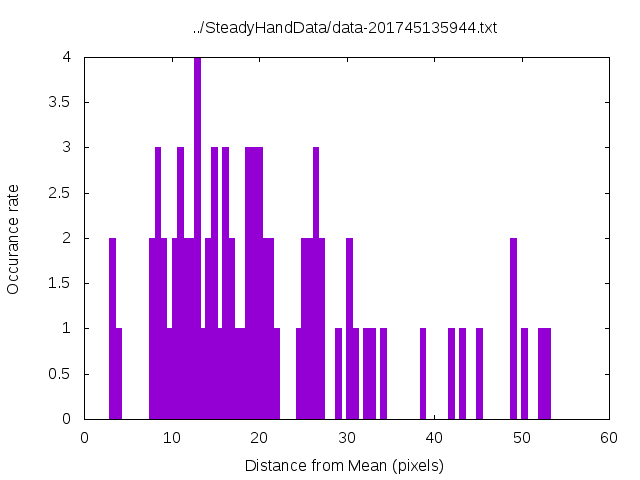
\includegraphics[scale=.5]{graph-data-201745135944.png}\\
\end{tabular}
\end{table}



\end{document}